\documentclass[12pt]{article}
\usepackage[top=3cm, left=3cm, right=3cm, bottom=2.5cm]{geometry}
\usepackage{amsmath,bm}
\usepackage{xcolor}
\usepackage{float}
\usepackage{graphicx}
\usepackage{nicefrac}
\usepackage{amsfonts}


\begin{document}

\title{FFF first calculations}
\author{Higor S. Monteiro}

\maketitle

Let us start with the $| n = 1, \ell = 1 \rangle$ fiber circuits. 
There are four possible synchronous configurations for this
type of circuit and only three are observed in the \textit{E.Coli} 
genetic regulatory network (Fig.~\ref{fig:fig1}). Following the notations
of \cite{ian_coupled_bifur}, we denote the networks of Fig.~\ref{fig:fig1} as 
\textbf{biological} networks. However, to use the formalism of coupled cell networks
\cite{coupled-cell} we first derive a new form of network from the original
ones in Fig.~\ref{fig:fig1}. This way, for each gene $x$ with internal dynamics $x(t)$
we divide it into two new nodes $x^R$ and $x^P$ representing different variables
related to the expression rate dynamics of gene $x$: the concentration $x^R$ of
the mRNA and the concentration $x^P$ of its associated protein. Then, we define
the regulations only between different nodes in the new network according to the
pattern of regulations in the biological network. This 
derivation is displayed in Fig.~\ref{fig:fig2} for the Feed-Forward Fiber (FFF).
We denote the new network as \textbf{mathematical} network.

\begin{figure}[H]
    \centering
    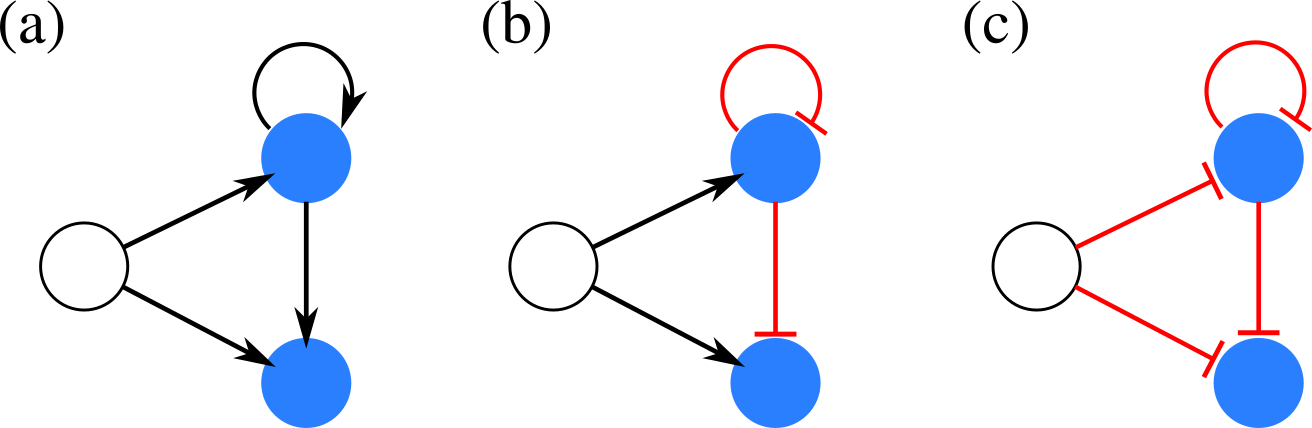
\includegraphics[scale=0.44]{drawings/fig1.png}
    \caption{Observed $| n = 1, \ell = 1 \rangle$ fiber circuits in \textit{E.Coli} network.}
    \label{fig:fig1}
\end{figure}

\begin{figure}[H]
    \centering
    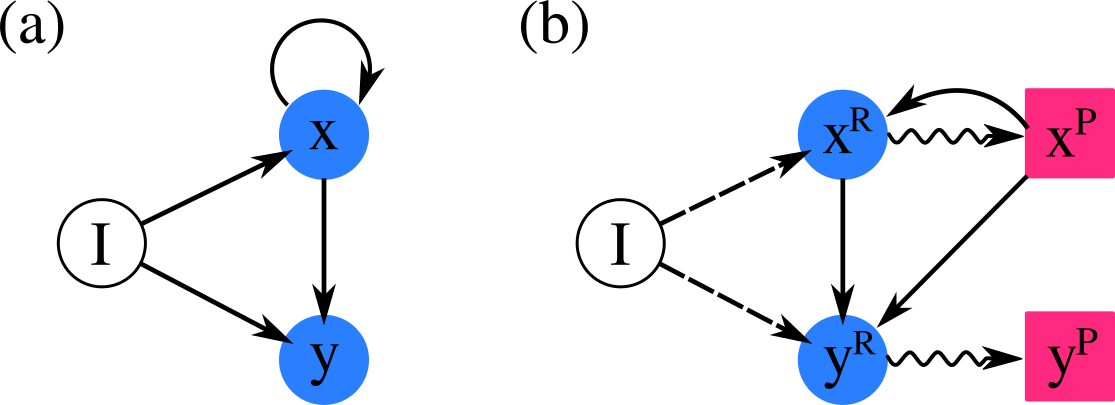
\includegraphics[scale=0.48]{drawings/fig2.png}
    \caption{(a) Biological network representation. (b) Mathematical network representation.}
    \label{fig:fig2}
\end{figure}

After we define the proper mathematical network for a given circuit, we can 
define the general form of the admissible equations of the network. In our case,
nodes with superscripts $R$ and $P$ are considered as distinct types of nodes and,
therefore, have different internal dynamics. The dynamics of the mRNA and protein
nodes are represented by the $f$ and $g$ functions, respectively. Since the 
admissible equations do not consider the types of each regulation (activator 
or repressor) we can use the pattern of regulations of the network in 
Fig.~\ref{fig:fig2}(b) to write the following system for all the 
$|n=1,\ell = 1 \rangle$ circuits:
\begin{equation} \label{eq:sys-eq}
    \begin{aligned}
        \dot{x}^R &= f(x^R, x^P, I)\\
        \dot{x}^P &= g(x^P, x^R)\\
        \dot{y}^R &= f(y^R, x^P, I)\\
        \dot{y}^P &= g(y^P, y^R),
    \end{aligned}
\end{equation}
where the vector of coordinates is $(x^R, x^P, y^R, y^P)$.

Next, we calculate the Jacobian of the system of equations of Eq.~\ref{eq:sys-eq} 
where we define the following notation: $\nicefrac{\partial f}{\partial x^i} = f_j$ 
such that $j$ is the position of the variable $x^i$ in the dependence of $f$. 
For instance, we have $\nicefrac{\partial f}{\partial x^R} = f_1$ and 
$\nicefrac{\partial f}{\partial x^P} = f_2$ for node $x^R$. The same notation 
goes for the dynamics of $g$. Therefore, we obtain for the Jacobian:
\begin{equation}
    J = \begin{pmatrix}
        \nicefrac{\partial f}{\partial x^R} & \nicefrac{\partial f}{\partial x^P} &
        \nicefrac{\partial f}{\partial y^R} & \nicefrac{\partial f}{\partial y^P} \\
        % line 2
        \nicefrac{\partial g}{\partial x^R} & \nicefrac{\partial g}{\partial x^P} &
        \nicefrac{\partial g}{\partial y^R} & \nicefrac{\partial g}{\partial y^P} \\
        % line 3
        \nicefrac{\partial f}{\partial x^R} & \nicefrac{\partial f}{\partial x^P} &
        \nicefrac{\partial f}{\partial y^R} & \nicefrac{\partial f}{\partial y^P} \\
        %line 4
        \nicefrac{\partial g}{\partial x^R} & \nicefrac{\partial g}{\partial x^P} &
        \nicefrac{\partial g}{\partial y^R} & \nicefrac{\partial g}{\partial y^P}
    \end{pmatrix} = 
    \begin{pmatrix}
        f_1 & f_2 & 0 & 0 \\
        g_2 & g_1 & 0 & 0 \\
        0 & f_2 & f_1 & 0 \\
        0 & 0 & g_2 & g_1 
    \end{pmatrix}
\end{equation}

\begin{figure}[H]
    \centering
    
\includegraphics[scale=0.65]{drawings/fig3.png}
    \caption{Base network of the original mathematical network.}
    \label{fig:fig3}
\end{figure}

The synchrony subspace $\Delta$, determined by the balanced coloring of the
mathematical network, is given as $\Delta = \{ \bm{x} \in \mathbb{R} \ | \ 
\bm{x} = (u, v, u, v) \}$ where we have assumed $x^R = y^R = u_0$ and 
$x^P = y^P = v_0$ for the synchronous equilibrium. For the synchronous
equilibrium we have $f_1 = a$, $f_2 = b$, $g_1 = c$, $g_2 = d$, which sets 
the Jacobian as 
\begin{equation}
    J = \begin{pmatrix}
        a & b & 0 & 0\\
        d & c & 0 & 0\\
        0 & b & a & 0\\
        0 & 0 & d & c\\
    \end{pmatrix}.
\end{equation}
The main calculation is to use the Jacobian above to find what are the conditions for 
bifurcations and what are the types of these bifurcations. Using the discussion provided 
by Prof. Ian in his notes, we have stable synchrony-preserving bifurcations for $a < 0$ 
and $c < 0$. Also, synchrony-breaking steady-state bifurcation exists if $f_1g_1 = 0$. According to 
\cite{ian_coupled_bifur}, synchrony-breaking bifurcations occur when a synchronous state loses 
stability and bifurcates to a state with less synchrony.

After we found the bifurcation conditions, we need to relate the Jacobian $J$ with 
the parameters of the chosen special model used for each combination of activator/repressor 
regulations. In Fig.~\ref{fig:fig3} we observe the quotient(base) network of the 
mathematical network of Fig.~\ref{fig:fig2}(b).

\textbf{First case} to analyze is for the FFF with all regulations positive. The continuous 
model in the base network is given by
\begin{equation}
    \begin{aligned}
        f(u,v,I) & = -\delta u + (1 - S(v)) + I\\
        g(u,v) & = -\alpha u + \beta v
    \end{aligned},
\end{equation}
where $S(v)$ is the Hill function for some exponent $n$, and $I$ is some input independent
of the expression rates of $u$ and $v$. Then, we compare the parameters of the special 
model with the values of the Jacobian. Since $\delta$, $\alpha$ and $\beta$ are positive 
parameters (degradation and production rates), we obtain that: $f_1 = \nicefrac{\partial f}{\partial u} 
= -\delta < 0$, $f_2 = \nicefrac{\partial f}{\partial v} = -S'(v) > 0$, $g_1 = 
\nicefrac{\partial g}{\partial u} = - \alpha < 0$, 
$g_2 = \nicefrac{\partial g}{\partial v} = \beta > 0$. Therefore, according to Ian's note, the bifurcation ($f_1 < 0$ 
and $g_1 < 0$) is {\color{red}synchrony-preserving}.


For the discussion of the \textbf{second case}, we observe that if the input 
$I$ does not have any dependence on either $u$ or $v$, 
then the UNSAT-FFF circuits displayed in Fig.~\ref{fig:fig1}(b) and (c), where the external 
regulator is either a repressor or an activator, are equivalent, and the equations 
for the continuous model considered are identical for both
\begin{equation}
    \begin{aligned}
        f(u,v,I) & = -\delta u + S(v) + I\\
        g(u,v) & = -\alpha u + \beta v
    \end{aligned},
\end{equation}
where again $f_1 = -\delta < 0$ and $g_1 = -\alpha < 0$, which indicates that the bifurcation 
is also {\color{red}synchrony-preserving}. Although $g_2 = \beta$ just as the first case, $f_2$
is this time different, assuming a negative value: $f_2 = \nicefrac{\partial f}{\partial v} = S'(v) < 0$.

%\begin{bibliography}{1}
%
%\bibitem{ian_coupled_bifur} 
%M. Golubitsky*, M. Pivato and I. stewart 
%\textit{Interior symmetry and local bifurcation in
%coupled cell networks}. 
%Dynamical Systems, 4(19):389–407, 2004 
%
%\end{bibliography}

\end{document}